\chapter{Introduction}\label{chap:introduction}
In this project an industrial robot is automated to manufacture certain characters from The Simpsons family using Lego Duplo bricks \cite{duplo}. The choice of characters that are produced by the robot include Homer, Marge, Bart, Lisa and Maggie. Each character is made using a specific order and color of the bricks. Each character is produced using three Duplo bricks besides Maggie, which is produced using only two Duplo bricks. The specifications of each character is given below and shown in \autoref{fig:lego_simpsons}.:

\begin{itemize}
	\item Homer: blue, black and yellow.
	\item Marge: green, yellow and blue.
	\item Bart: blue, orange, yellow.
	\item Lisa: yellow, orange, yellow.
	\item Maggie: blue, yellow.
\end{itemize}

\begin{figure}[H]
    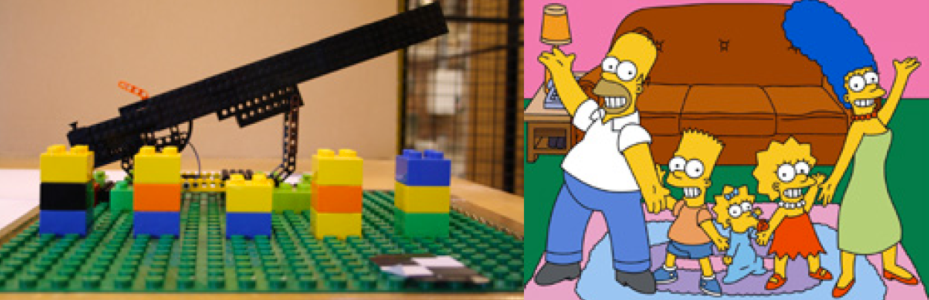
\includegraphics[width=0.6\textwidth]{figures/lego_simpsons.pdf}
    \caption{Image showing The Simpsons family produced with Lego Duplo bricks besides an image of the actual Simpsons family.}
    \label{fig:lego_simpsons}
\end{figure}

The task presented is an ideal example of a process that should be automated. Automation plays a key role in production and manufacturing as it contributes to reducing production costs while improving product quality and reducing production time. Generally, industrial robots are used for repetitive tasks, such as the one presented. The robot chosen for this task is the KUKA KR6 700 \cite{kuka}.

In order to automate this procedure, the task is broken down into two main sections, namely, computer vision and robot manipulation. Computer vision is needed to recognize the bricks in the workspace. The properties that define a brick are its color, location and orientation. A USB camera is placed above the bricks' workspace and image processing techniques are used to classify the bricks' properties. The algorithm also translates the orientation and location of the bricks from the image's coordinate frame to the robot's coordinate frame.

Once the bricks are classified, an algorithm calculates which bricks must be used for each figure and then sends commands the robot to pick and place the bricks, one at a time. To pick up the Lego bricks a gripper is designed and 3D printed such that the robot grabs the bricks with two opposite corners, thus ensuring the orientation of the brick in the gripper is precisely known. This is needed to accurately place the bricks on top of each other when producing the figures. First a command is given to the robot to move to the location of the required brick and then a command to close the gripper on the brick is sent. The robot is then given a command to place the brick on a green Lego Duplo grid, on which the characters are produced.

This procedure is fully automated, and the only input the robot receives is the number of each character needed, as specified by the user. The robot starts in its home position and then returns back to its home position after manufacturing the specified figures.



% This involves among other things:
% \begin{itemize}
%     \item Identifying which bricks are located on the table.
%     \item Identifying the location of the bricks (e.g. the location of a black Dublo brick needed to build Homer)
%     \item Determine the associated cost of each solution and the cheapest solutions.
%     \item Grasping the bricks by means of a robot.
%     \item Mounting the bricks on a plate or on top of other bricks
%     \item Selecting the sequence in which you want to pick/place the bricks and build the figures.
% \end{itemize}